%!TEX root = Main.tex

\appendix

\section{Appendix section}\label{app}

TO DO:
\begin{enumerate}
\item Combine multiple subjects.
\item Visualization: mean intensity.
\item Reading: basic knowledge about point process, and shift operation, identifiability.
\item Literature review.
\item Sketch of proof.
\item Real data.
\item Selection of k.
% \item Convex relaxation/FPCA (reading).
\end{enumerate}

\subsection{Plots}
\begin{figure}[H]
\begin{subfigure}{.8\textwidth}
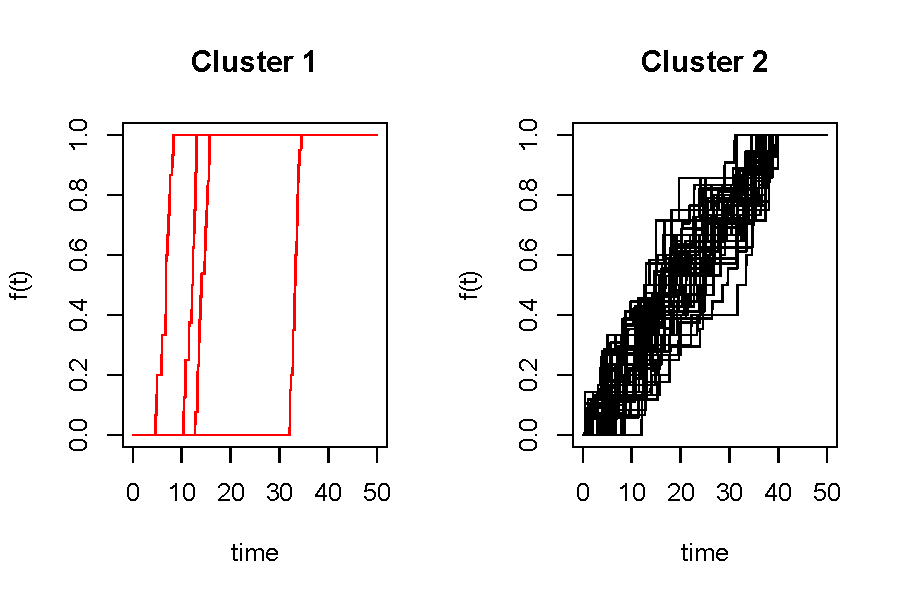
\includegraphics[width=\linewidth]{../simulation/plots/f_list_1}
\caption{}
\label{fig: original curves}
\end{subfigure}
\begin{subfigure}{.8\textwidth}
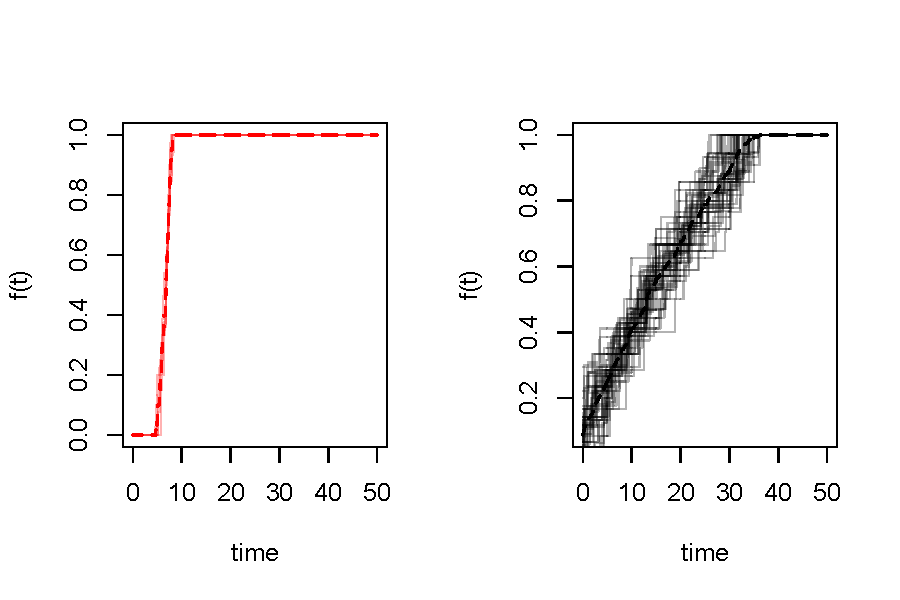
\includegraphics[width=\linewidth]{../simulation/plots/clus_results_1}
\caption{}
\label{fig: aligned curves}
\end{subfigure}
\caption{Case 1. (a): Empirical distribution functions before alignment. The red curves correspond to type I nodes, and the black curves correspond to type II nodes. (b): Clustering result. Solid lines represent the shifted distribution functions of nodes belonging to that cluster. The mean curves are plotted by dashed lines. }
\end{figure}



\begin{figure}[H]
\begin{subfigure}{.8\textwidth}
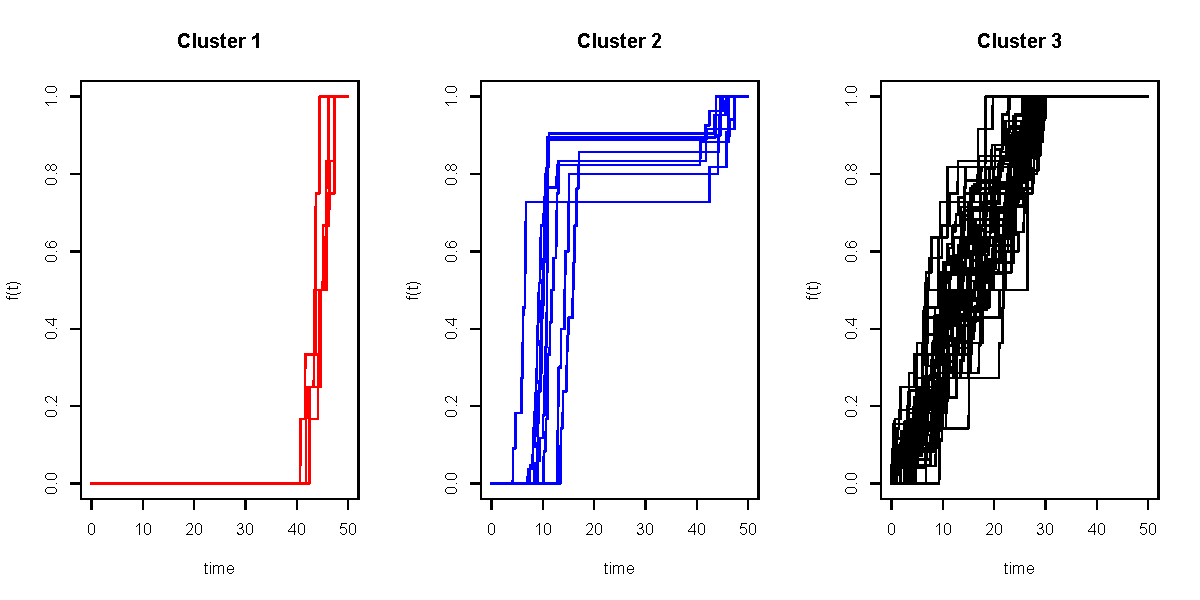
\includegraphics[width=\linewidth]{../simulation/plots/f_list_2}
\caption{}
\label{fig: original curves, case 2}
\end{subfigure}
\begin{subfigure}{.8\textwidth}
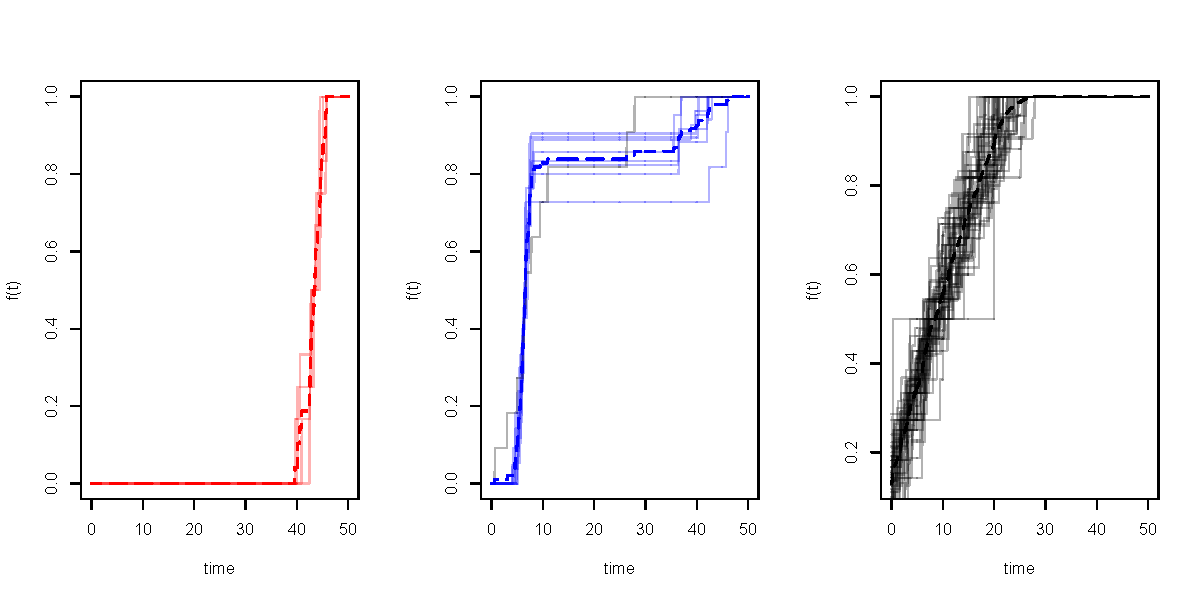
\includegraphics[width=\linewidth]{../simulation/plots/clus_results_2}
\caption{}
\label{fig: aligned curves, case 2}
\end{subfigure}
\caption{Case 2. (a): Empirical distribution functions before alignment. The red, blue and black curves correspond to type I, II, III nodes, respectively. (b): Clustering result. Solid lines represent the shifted distribution functions of nodes belonging to that cluster. The mean curves are plotted by dashed lines. }
\end{figure}




\begin{figure}[H]
\begin{subfigure}{.8\textwidth}
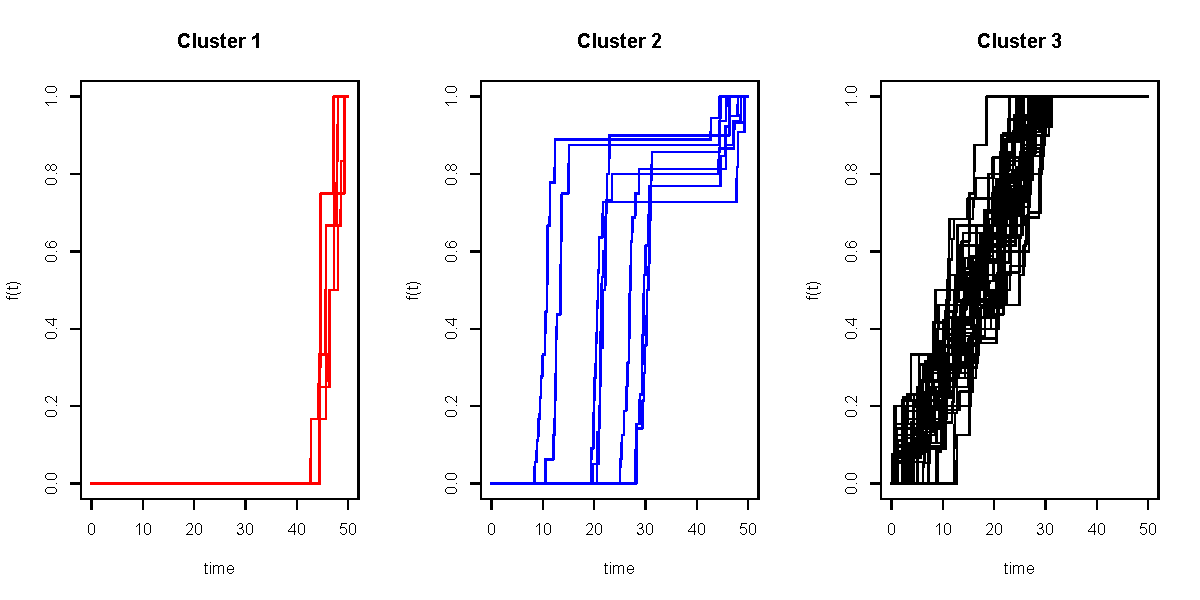
\includegraphics[width=\linewidth]{../simulation/plots/f_list_3}
\caption{}
\label{fig: original curves, case 3}
\end{subfigure}
\begin{subfigure}{.8\textwidth}
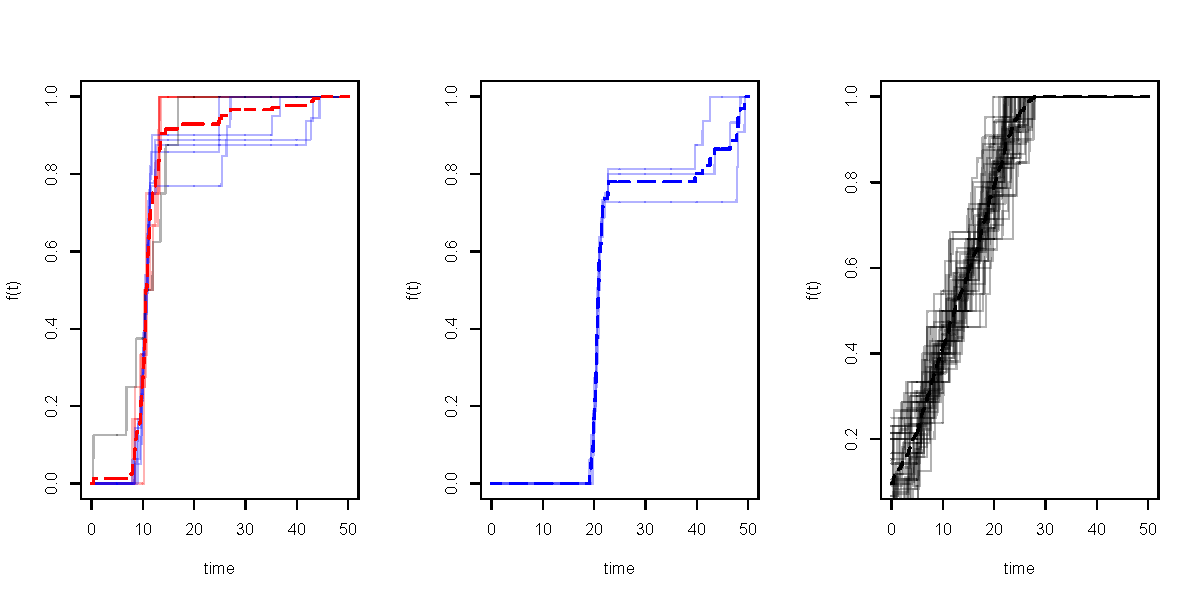
\includegraphics[width=\linewidth]{../simulation/plots/clus_results_3}
\caption{}
\label{fig: aligned curves, case 3}
\end{subfigure}
\caption{Case 3. (a): Empirical distribution functions before alignment. The red, blue and black curves correspond to type I, II, III nodes, respectively. (b): Clustering result. Solid lines represent the shifted distribution functions of nodes belonging to that cluster. The mean curves are plotted by dashed lines. }
\end{figure}



% See Appendix \ref{app}.
